\documentclass[a4paper,11pt]{ltjsarticle}
\usepackage{geometry,enumitem,graphicx,float,caption,hyperref}
\geometry{margin=25mm}
\hypersetup{colorlinks=true,urlcolor=blue,linkcolor=black}
\title{外国人が増えた町で、参政党は伸びたのか}\author{}\date{}
\begin{document}
\maketitle

\href{https://note.com/good_nerine4177/n/na1c20fd7e763}{前回の記事}では、参政党の投票者に外国人の受け入れに否定的な人が多いことを確かめました。では、その否定的な気持ちはどこから来たのでしょうか。考えられる説を五つ挙げます。

\begin{itemize}[nosep]
\item 身近で外国人が増え、暮らしの変化を肌で感じた
\item 自分の町ではなく、近くの町で外国人が増えたのを見聞きした
\item 外国人の中でも、仕事で競合しやすい人たちが増えた
\item 観光客が増え、混雑などを目にした
\item 地域の事情とは関係のない、全国に共通する要因
\end{itemize}

もし最初の四つのどれかが正しければ、外国人や観光客が増えた地域ほど参政党は伸びたはずです。そこで、全国の市区町村のデータで確かめました。

\section*{使ったデータ}

2022年と2025年の参院選比例で、参政党の得票率がどれだけ伸びたかを、市区町村ごとに比べました。

\begin{itemize}[nosep]
\item 選挙の結果は総務省の開票区別の表。政令市は区を単位にし、全国1,883の単位
\item 外国人の割合は、住民基本台帳の外国人住民の数を総人口で割ったもの(2022年と2025年の1月1日)。国籍と在留資格の内訳は在留外国人統計
\item 観光は観光庁の宿泊旅行統計(都道府県別の外国人延べ宿泊者数)
\item 高齢者の割合や産業などの地域の特徴は、統計センターの市区町村データ
\item 個人の単位の確認には、前回と同じ東大谷口研・朝日2026年有権者調査
\end{itemize}

2025年の総務省の表では、豊橋市など16の開票区の数字が空欄でした。これらは県の合計から差し引いて補い、同じ県の空欄は一つの単位にまとめました。1,883の単位には、このまとめた3つの単位も含まれます。補った後の参政党の得票の合計は、公式の全国計と一致します。まとめた単位を除いても、結果はほとんど変わりません。

\section*{先行する分析}

外国人と参政党の得票の関係は、すでに何人かが調べています。

\begin{itemize}[nosep]
\item \href{https://uaz-pr.com/2025/12/25/20251228uaz_02/}{眞下英二氏(尚美学園大学)}は、全国の統計では外国人の数が得票に影響した証拠はないとしつつ、北関東やニセコなど外国人との共生が話題になる地域では影響した可能性があると述べています。
\item \href{https://todo-ran.com/t/kiji/25987}{とどラン}は都道府県別に、「外国人研修生・技能実習生数」とは正の相関(0.42)、「在日外国人」の数とは相関がない(0.15)と報告しています。
\item \href{https://note.com/clever_eel2325/n/nad1dfadd9601}{S\_KUMA氏}は2026年衆院選の東京23区で、外国人の割合が高い区ほど参政党の得票率が高いと報告しています。
\end{itemize}

いずれも、ある時点の外国人の「多さ」と得票を比べたものです。この記事では、外国人の「増え方」と得票の「伸び」を比べ、さらに外国人の種類や観光客も分けて見ます。

\section*{外国人の増え方では、伸びの差を説明できなかった}

参政党の得票率は、全国で3.3\%から12.5\%へと9.2ポイント伸びました。市区町村を外国人の増え方で20の群に分けても、伸びはどの群も8.4〜9.9ポイントで、ほぼ水平に並びます(図1)。

ある時点の多さで比べると、外国人の割合が高い地域ほど参政党の得票率はやや高く(1ポイントあたり0.1〜0.2ポイント)、S\_KUMA氏による先行する分析と同じ向きです。しかし、この3年間に外国人が増えた地域ほど伸びた、という関係は見られません。

\begin{figure}[H]\centering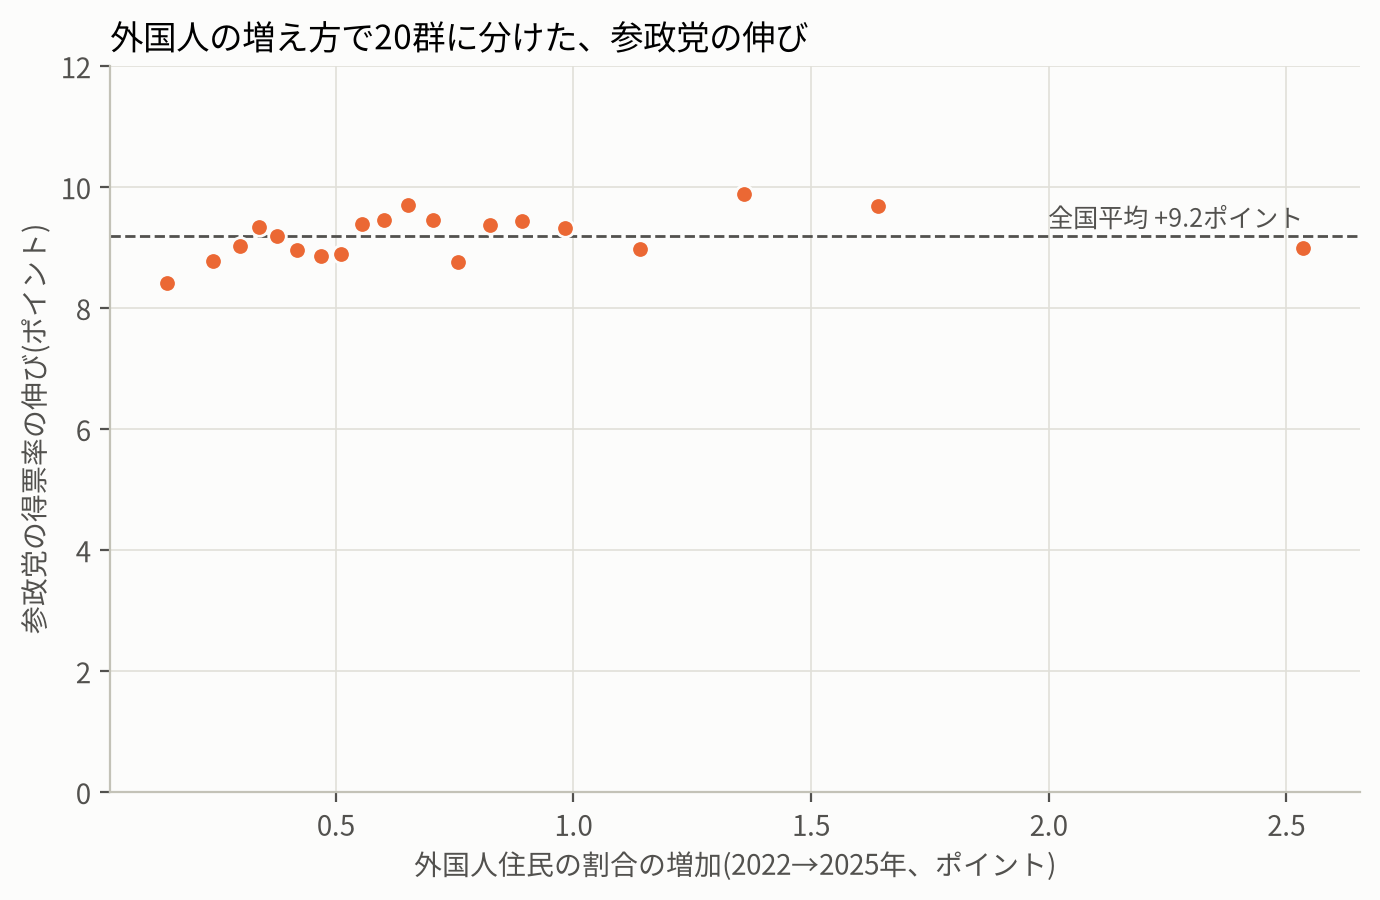
\includegraphics[width=\linewidth,height=0.8\textheight,keepaspectratio]{images/geo_binned.png}\caption*{\small 図1: 外国人住民の割合の増え方(2022→2025年)で市区町村を20群に分けた、参政党の得票率の伸び。破線は全国の伸び}\end{figure}

外国人の割合が1ポイント増えたときの伸びの違いを推定しても、同じでした(図2)。地域の特徴をそろえた推定で+0.2ポイントほどです。外国人の割合の増加は平均0.8ポイントなので、伸び全体のうち外国人の増加で説明できるのは2\%ほどです。区間の上の端を使っても3\%ほどにとどまります。

推定の向きは、2022年の外国人の割合をそろえるかどうかで変わります。外国人がもともと多い地域と、その後に増えた地域は同じではないからです。2022年の割合をそろえると「同じくらい外国人がいた地域どうしで、その後に増えたかどうか」の比較になり、係数は0近くまで下がります。

外国人が集まりやすい地域には、もともと別の特徴があるかもしれません。そこで補助的に、国籍ごとの全国での増え方を2015年の各地域の国籍構成で割り振った「予想される増え方」を使う推定(操作変数法)もしました。ただし、2015年の国籍構成は地域の産業などとも結びついています。実際、この予想値は2022年の参政党の得票率とも関係していました。また、結果は特定の国籍の扱いで大きく変わります。このため、この推定は確かな因果の証拠ではなく、効果が大きくないことを確かめる補助にとどまります。

役場の間の距離が10km以内の近くの町で外国人が増えたことも、伸びとの関係は同じく小さく、向きも安定しませんでした。

\begin{figure}[H]\centering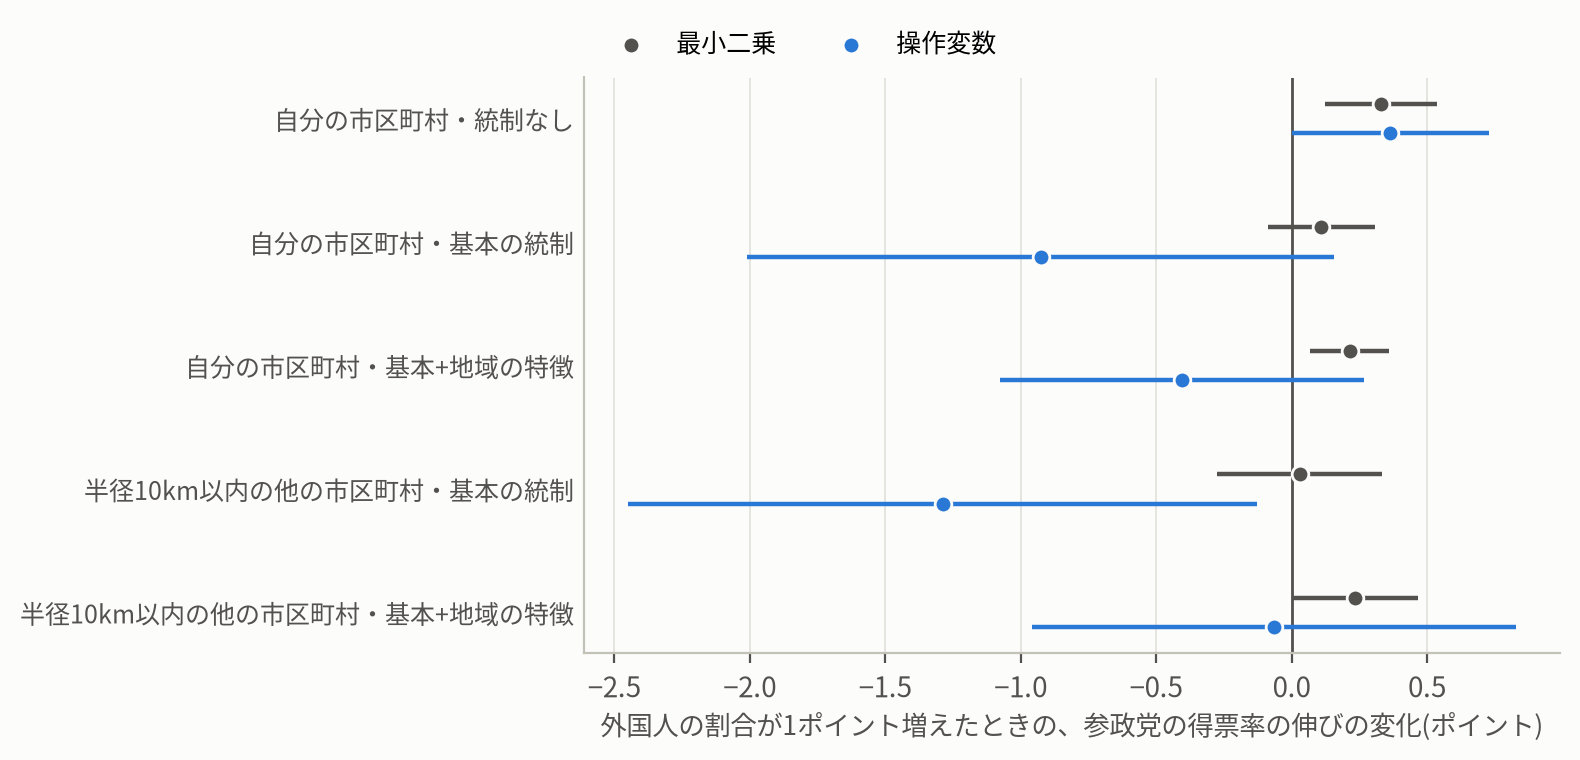
\includegraphics[width=\linewidth,height=0.8\textheight,keepaspectratio]{images/geo_effects.png}\caption*{\small 図2: 外国人の割合が1ポイント増えたときの、参政党の伸びの違い。線は95\%区間で、0をまたげばはっきりした差があるとは言えない。灰色は普通の回帰、青は操作変数法。2025年の有効投票数で重みをつけた}\end{figure}

個人の単位でも、関係は見えませんでした。東大・朝日調査の回答者に、住んでいる都道府県の外国人の割合と増え方を当てはめ、年代と性別をそろえて見ました。外国人労働者の受け入れ推進への反対、「在留外国人で文化が脅かされる」という答え、参政党への投票のどれとも、目立った関係はありませんでした。都道府県という粗い単位での確認です。

\section*{外国人の種類と観光客}

外国人の種類ごとの増加を同時に入れると、ベトナムと、その他の国籍(ミャンマーやスリランカなど)の増加が伸びと正の関係にありました(図3)。多くの種類を同時に調べたことを補正しても残る関係です。技能実習と特定技能も正の向きでしたが、補正すると、はっきりした差とは言えなくなります。これらの増加は人口の0.1〜0.2\%ほどなので、説明できる伸びはわずかです。

労働市場で日本人と分かれた仕事に外国人が集中するほど排外意識が強いという\href{https://www.jstage.jst.go.jp/article/jsr/63/1/63_19/_article/-char/ja}{永吉希久子氏の研究(2012年)}と、方向は合います。ただし、この分析は賃金や職種を測っていないので、仕事の中身が効いたとまでは言えません。産業など、外国人以外の地域の違いを拾っている可能性もあります。

\begin{figure}[H]\centering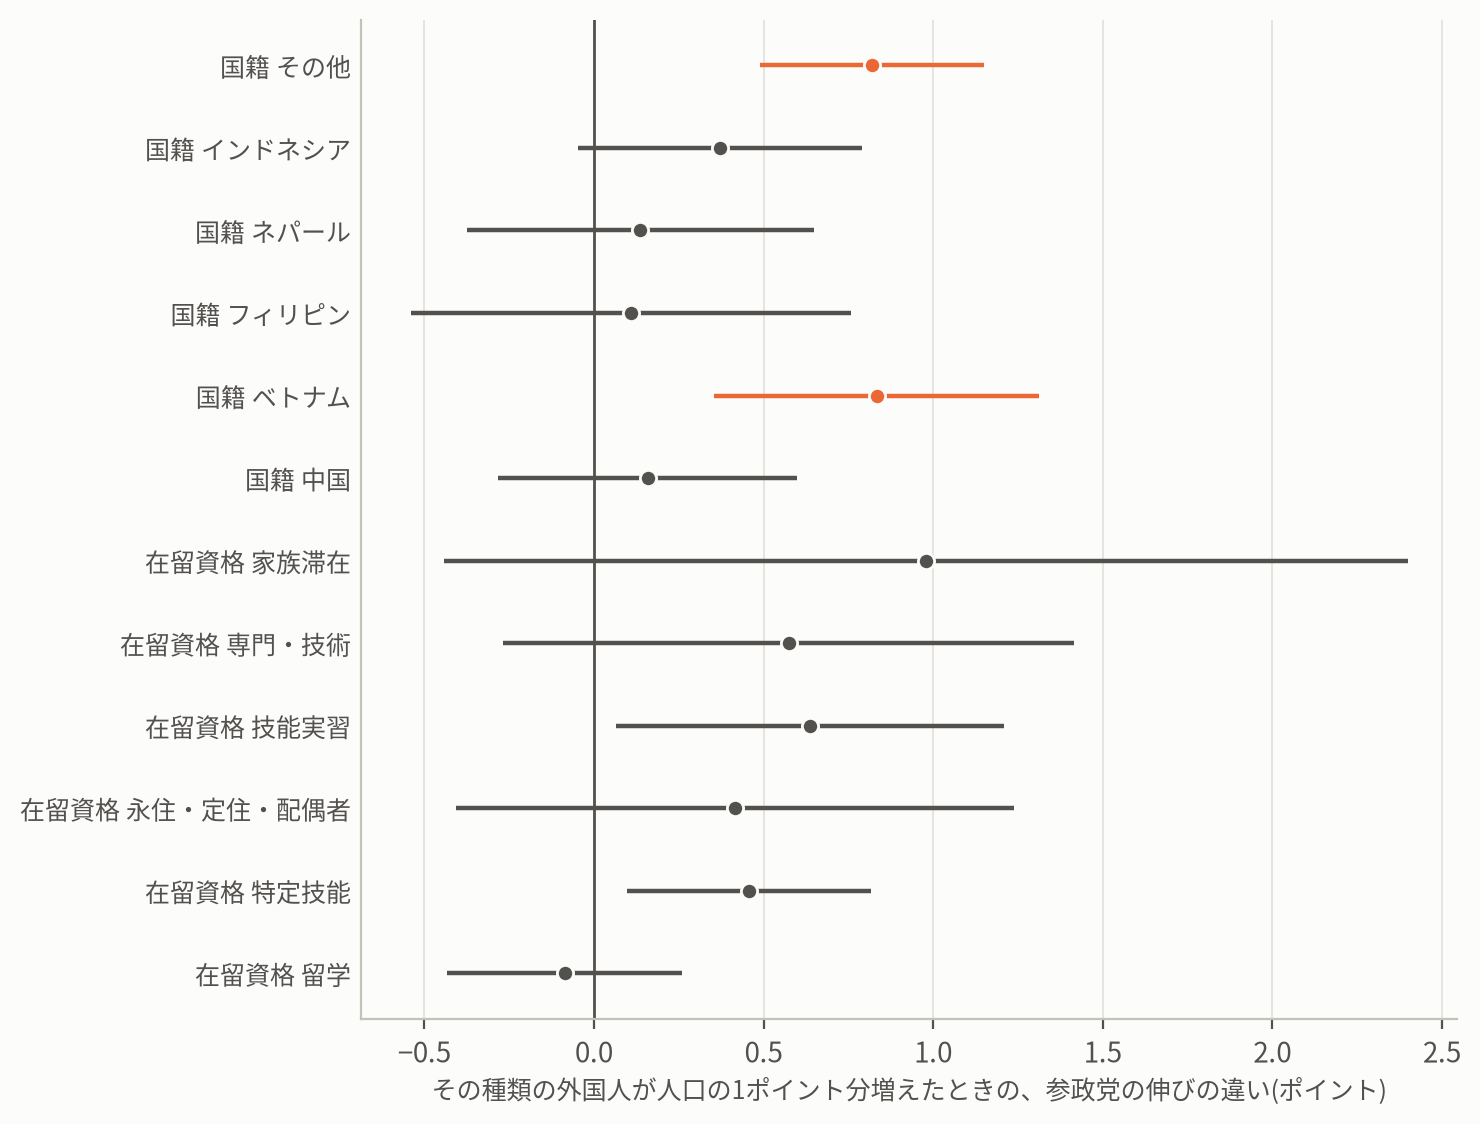
\includegraphics[width=\linewidth,height=0.8\textheight,keepaspectratio]{images/geo_groups.png}\caption*{\small 図3: 種類ごとの外国人の増加を同時に入れた推定(探索的な分析)。橙はHolm法で補正しても差が残るもの。地域の特徴をそろえた結果。増加がごく小さい種類は図から除いた}\end{figure}

観光客の多い都道府県で、参政党が特に伸びたわけでもありません(図4)。全体ではむしろ伸びが小さい傾向でしたが、これは東京、京都、沖縄、北海道の4都道府県によるもので、この4つを除くと関係は見えなくなります。47都道府県という少ない数での比較です。

\begin{figure}[H]\centering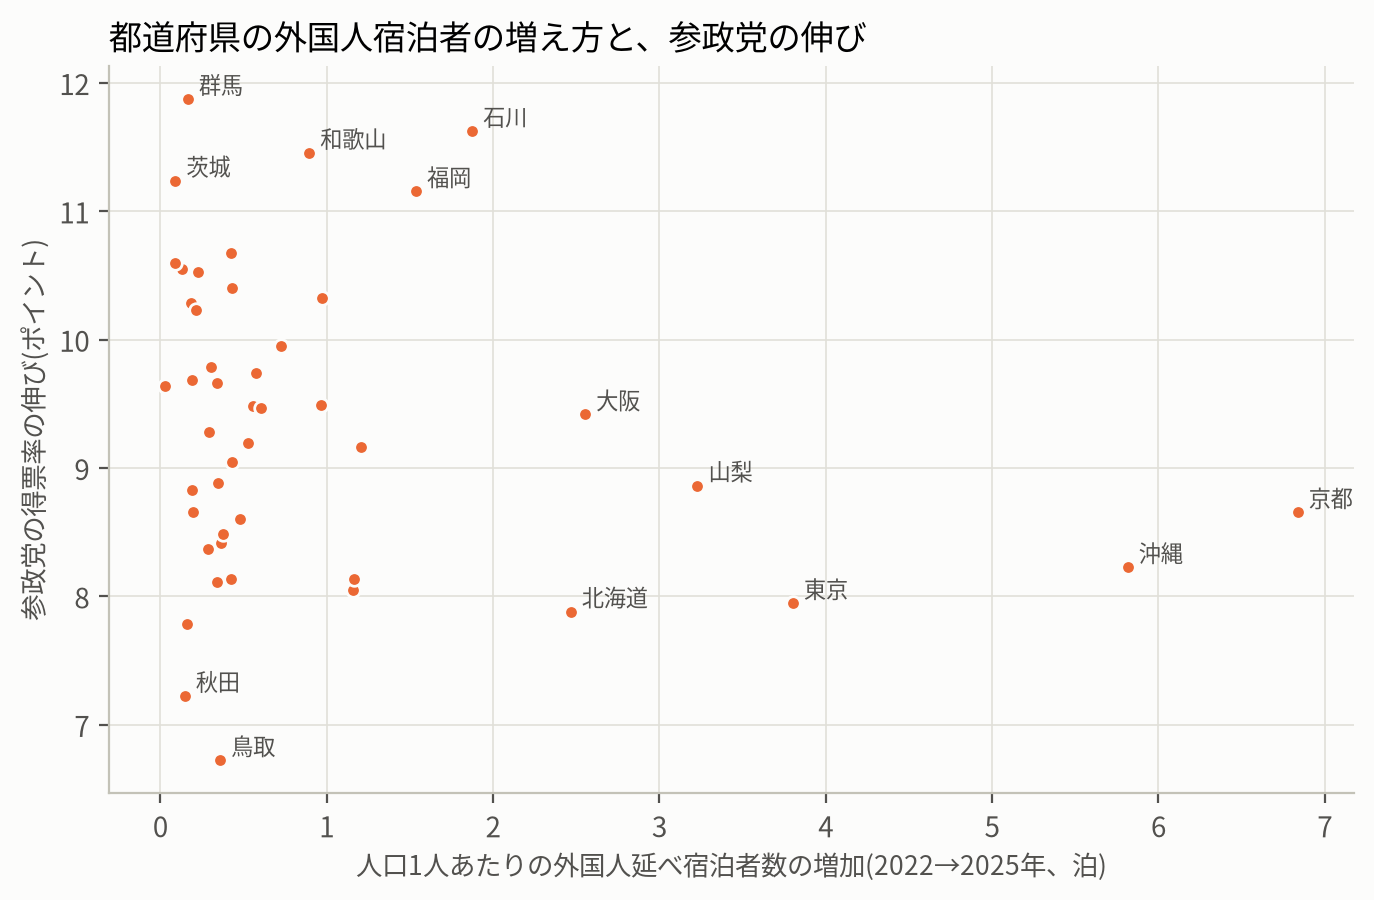
\includegraphics[width=\linewidth,height=0.8\textheight,keepaspectratio]{images/geo_tourism.png}\caption*{\small 図4: 都道府県の人口1人あたりの外国人延べ宿泊者数(2024年)と、参政党の伸び}\end{figure}

\section*{話題の町はどうだったか}

外国人の多さで話題になる町では、確かに伸びが全国平均を上回った所が多くあります。しかし、その多くは、外国人の変数を使わずに県・年齢構成・産業などから予想した伸びと、ほぼ同じでした(図5)。北関東の工業都市は、働く世代が多く、もともと伸びやすい地域です。外国人の割合が3年で6\%から19\%に増えたニセコ町は、全国平均も予想もわずかに下回りました。一方、隣の倶知安町は予想を4ポイント上回っており、一律ではありません。小さな町は票数が少なく、個別の上下には偶然も含まれます。

\begin{figure}[H]\centering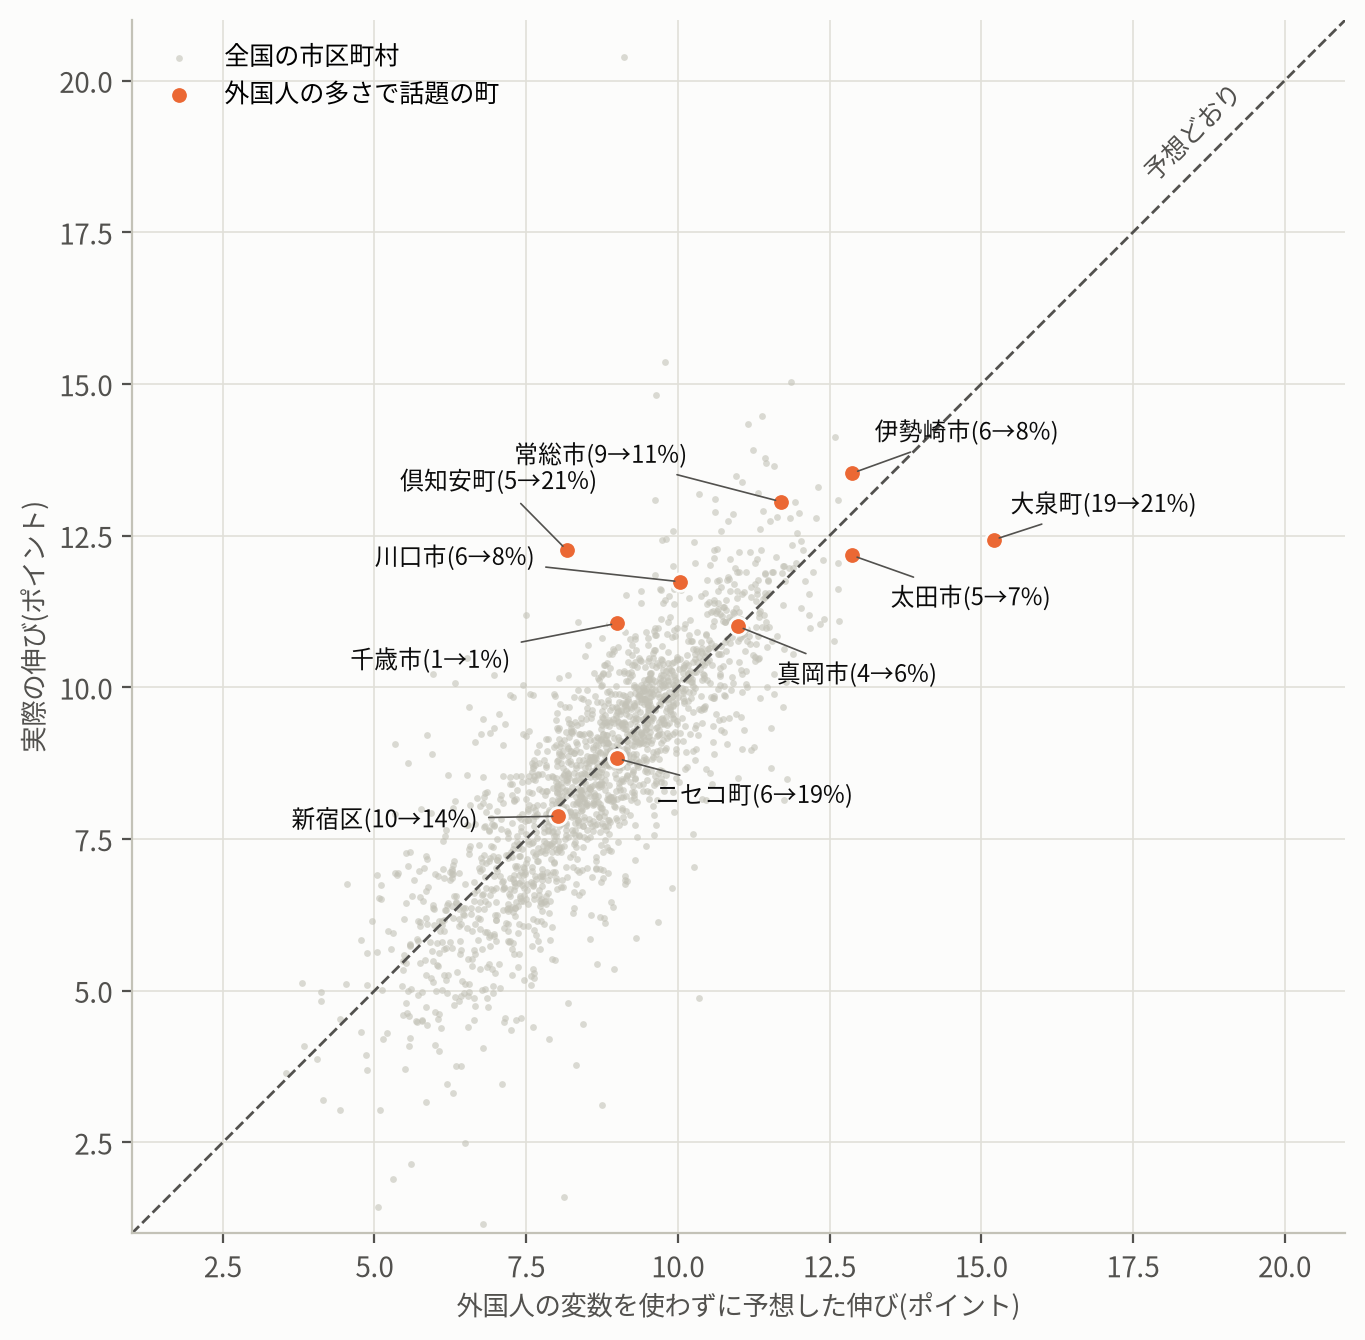
\includegraphics[width=\linewidth,height=0.8\textheight,keepaspectratio]{images/geo_places.png}\caption*{\small 図5: 外国人の多さで話題になる町の、実際の伸びと、外国人の変数を使わずに県・2022年の得票率・人口・年齢構成・産業などから予想した伸び}\end{figure}

\section*{地域差と最も強く結びついていたのは年齢構成}

伸びの地域差と最も強く結びついていたのは、高齢者の割合でした(図6)。高齢者の割合が低い地域ほど、参政党の伸びが大きい傾向があります。前回の記事で見た、投票者に40〜50代が多いという個人の結果とも矛盾しません。ただし、地域の年齢構成と投票者個人の年齢は別のものです。

\begin{figure}[H]\centering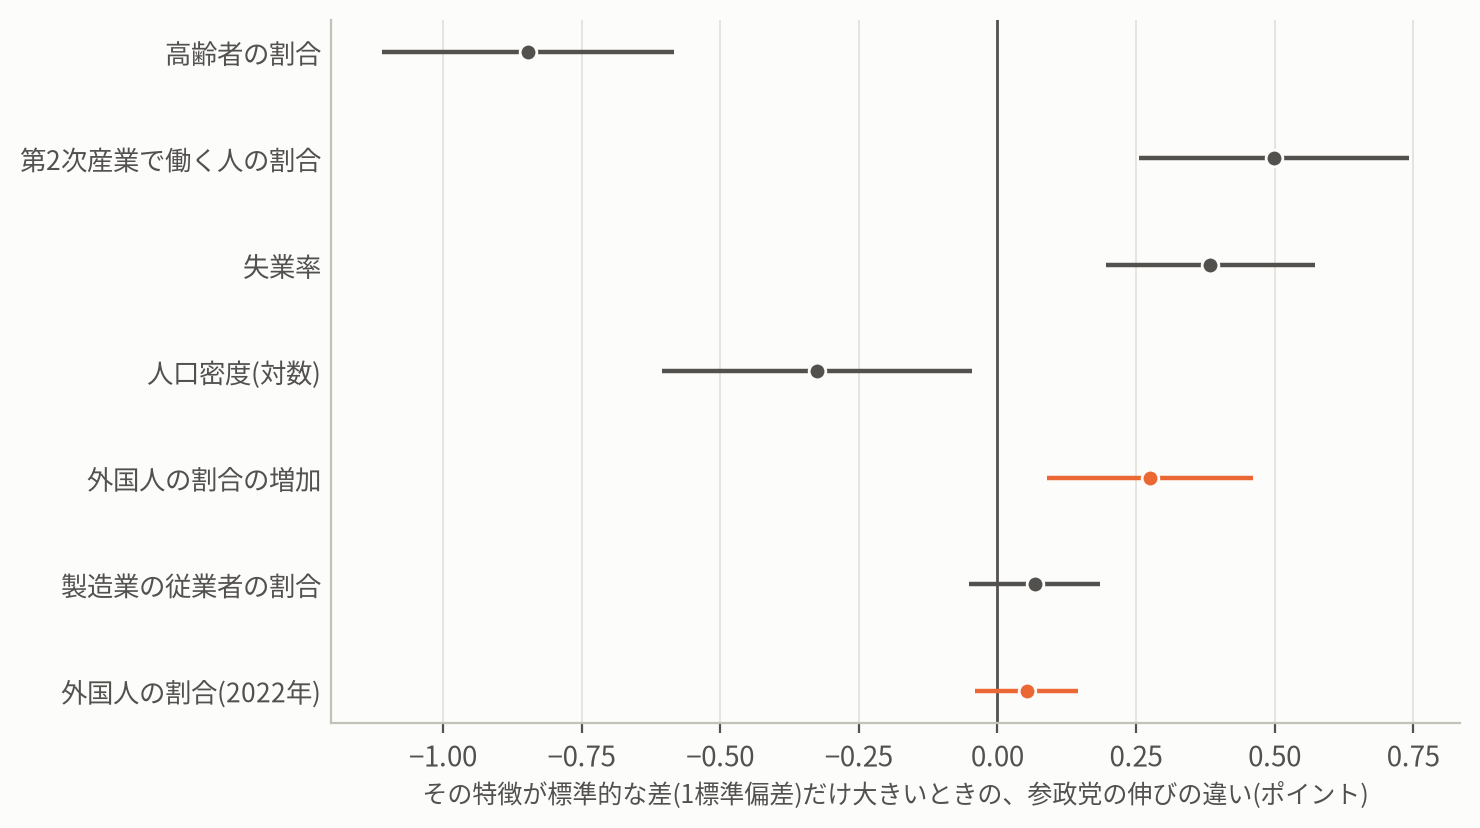
\includegraphics[width=\linewidth,height=0.8\textheight,keepaspectratio]{images/geo_drivers.png}\caption*{\small 図6: 地域の特徴を同時に入れたときの、参政党の伸びとの関係。特徴の標準的な差(1標準偏差)あたり}\end{figure}

この点で、参政党の伸びた地域は、れいわ新選組が強かった地域と重なります。2022年にれいわの得票率が1ポイント高かった地域では、参政党の伸びが0.4ポイント大きくなっていました。ただし、年齢構成などの地域の特徴をそろえると、この差は0.06ポイントとほぼ消えます。どちらも高齢者の少ない地域で強い、という共通点によるものです。地域の単位の結果なので、同じ人が両党に投票したことを示すわけではありません。それでも、前回の記事で見た両党の投票者の属性の近さとは矛盾しない結果です。

\section*{先行研究との関係}

身近な外国人の数が外国人への態度にどう影響するかについて、これまでの研究の結果は分かれています。

\begin{itemize}[nosep]
\item \href{https://ies.keio.ac.jp/upload/DP2021-005EN.pdf}{大久保敏弘氏(2021年、ディスカッションペーパー)}は、都道府県の外国人労働者の割合が移民への態度に効かないと報告しています。
\item \href{https://doi.org/10.1093/sf/soab115}{Laurence・五十嵐・石田各氏(2022年)}は、2008〜2014年に同じ人を追った調査で、住む都道府県の外国人の割合が上がると、移民の受け入れへの支持が下がると報告しています。ただし市区町村の単位では、この悪化は外国人の割合が7\%未満の地域に集中していました。外国人との接触が増えることが、悪化を和らげる方向に働いていたとしています。
\item \href{https://j-hai.github.io/assets/pdf/annualrev-imig-attitudes.pdf}{Hainmueller・Hopkins両氏(2014年)}は、各国の研究をまとめたレビューで、移民への態度は個人の経済状況とはあまり関係せず、国全体への文化的な影響への懸念、次いで経済的な影響への懸念で形づくられるとしています。
\item \href{https://kaken.nii.ac.jp/file/KAKENHI-PROJECT-25780305/25780305seika.pdf}{永吉氏の科研費の研究成果報告書(2016年)}は、外国人の集住地でも問題が「隣町」の話として伝聞で語られるという研究を引き、現実の競争より「想像された脅威」が反外国人感情を刺激していると考えるのが妥当だと述べています。
\item \href{https://doi.org/10.1525/as.2023.1922764}{Yin氏(2023年)}は要旨で、文化や治安についての懸念は、主に移民へのステレオタイプから生じていると述べています。
\end{itemize}

Laurenceらの結果と、この記事の結果は矛盾しません。向こうが見ているのは外国人への態度で、この記事が見ているのは参政党への票の伸びです。外国人が増えて態度がいくらか悪くなったとしても、それが参政党の伸びの地域差として表れるほどではなかった、と考えられます。

\section*{おわりに}

外国人が増えた町で、参政党が特に伸びたわけではありませんでした。外国人の増え方では伸びの地域差をほとんど説明できず、差と最も強く結びついていたのは年齢構成です。

前回の記事と合わせると、外国人の受け入れに否定的であることと、身近で外国人が増えたことに反応していることは、別のことだと分かります。五つの説のうち、データと矛盾しないのは最後の、全国に共通する要因です。仕事で競合しやすい外国人の増加は、正の向きの関係が一部に見えましたが、説明できる伸びはわずかでした。ただし、それが報道やSNSなのか、政治への不満なのか、党の活動なのかは、このデータでは分かりません。ほかの説が合わなかった結果として残る解釈です。

参政党の票は、人口とほぼ同じ割合で全国に散らばっています。2025年の票の87\%は、外国人の割合が5\%未満の地域から出ています。

ここからは私の感想です。身近に外国人が増えたわけでもないのに、外国人の問題を理由に一票を投じる。これは、地元の住民でもないのに全国から基地反対運動に駆けつける左派の運動と、同じ構図ではないでしょうか。右も左も、当事者でない人ほど熱くなるものなのかもしれません。

\section*{著作権について}

分析のコードは\href{https://github.com/hrkimura/seiryoku-shisu/tree/master/sanseito_geo}{GitHub}にMITライセンスで公開し、自由に使ってもらって構いません。ただしこの記事の文章そのものの著作権は放棄していません。東大・朝日調査の個票は再配布が禁じられているので、コードと一緒には公開していません。

\section*{AI活用について}

分析の設計・検証・実装と、この記事の下書きには、AI(Claude)を活用しています。

{\small この記事は東大谷口研・朝日調査データを使用しました。}
\end{document}
